\begin{apendicesenv}

\chapter{Rotina MatLab para cálculo do sistema sem fim}

\begin{figure}[H]
    \centering
      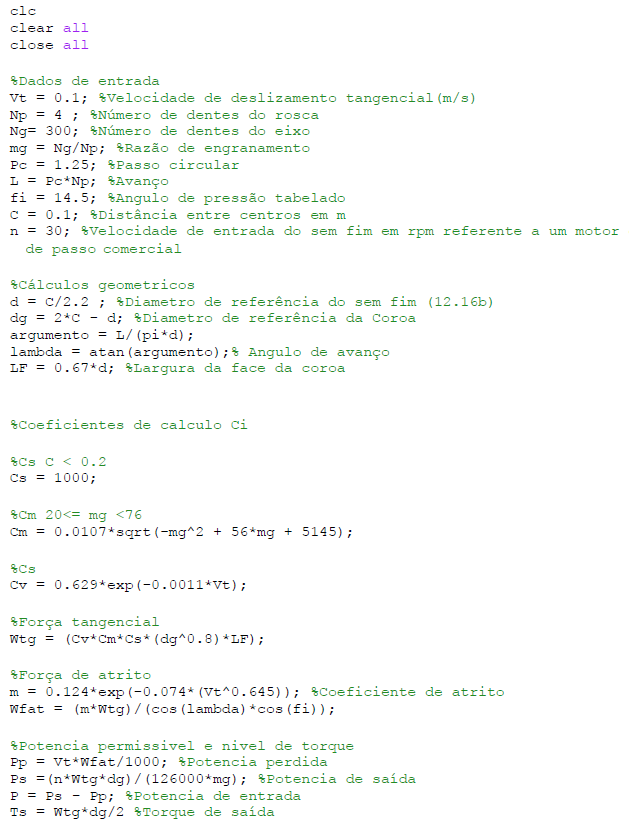
\includegraphics[scale=1.0]{figuras/matlabsemfim.png}
    \label{matlabsemfim}
\end{figure}

\chapter{Desenhos Técnicos}

\textbf{Componentes em x}

\begin{figure}[H]
    \centering
      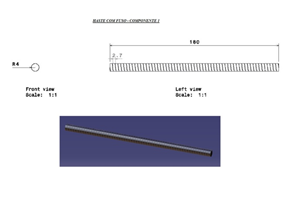
\includegraphics[scale=1.0]{figuras/tec1.png}
    \caption{Desenho Técnico componente 1}
    \label{tec1}
\end{figure}

\begin{figure}[H]
    \centering
      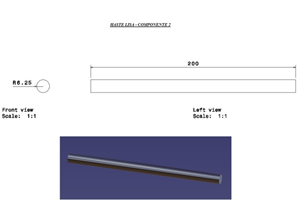
\includegraphics[scale=1.0]{figuras/tec2.png}
    \caption{Desenho Técnico componente 2}
    \label{tec2}
\end{figure}

\begin{figure}[H]
    \centering
      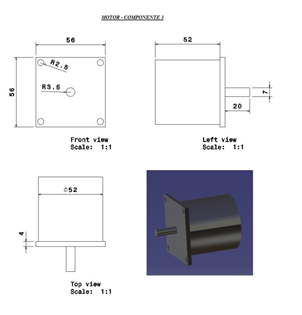
\includegraphics[scale=1.0]{figuras/tec3.png}
    \caption{Desenho Técnico componente 3}
    \label{tec3}
\end{figure}

\begin{figure}[H]
    \centering
      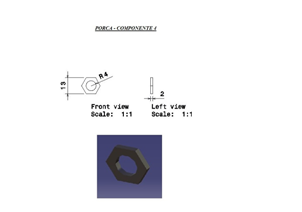
\includegraphics[scale=1.0]{figuras/tec4.png}
    \caption{Desenho Técnico componente 4}
    \label{tec4}
\end{figure}

\begin{figure}[H]
    \centering
      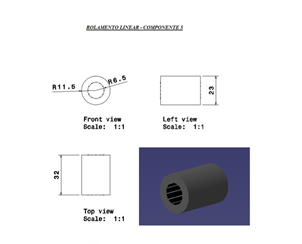
\includegraphics[scale=1.0]{figuras/tec5.png}
    \caption{Desenho Técnico componente 5}
    \label{tec5}
\end{figure}

\begin{figure}[H]
    \centering
      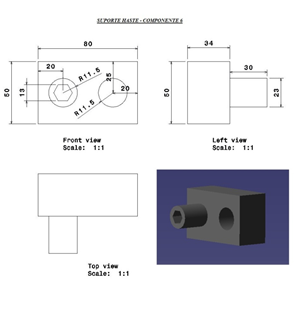
\includegraphics[scale=1.0]{figuras/tec6.png}
    \caption{Desenho Técnico componente 6}
    \label{tec6}
\end{figure}

\begin{figure}[H]
    \centering
      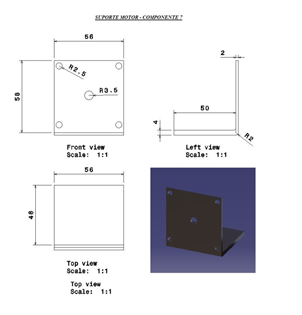
\includegraphics[scale=1.0]{figuras/tec7.png}
    \caption{Desenho Técnico componente 7}
    \label{tec7}
\end{figure}

\begin{figure}[H]
    \centering
      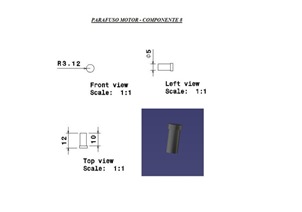
\includegraphics[scale=1.0]{figuras/tec8.png}
    \caption{Desenho Técnico componente 8}
    \label{tec8}
\end{figure}

\begin{figure}[H]
    \centering
      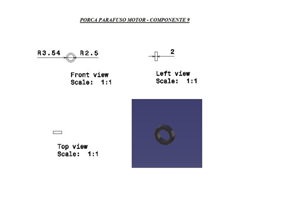
\includegraphics[scale=1.0]{figuras/tec9.png}
    \caption{Desenho Técnico componente 9}
    \label{tec9}
\end{figure}

\begin{figure}[H]
    \centering
      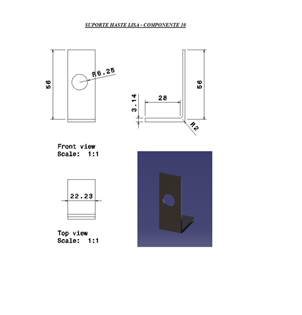
\includegraphics[scale=1.0]{figuras/tec10.png}
    \caption{Desenho Técnico componente 10}
    \label{tec10}
\end{figure}

\begin{figure}[H]
    \centering
      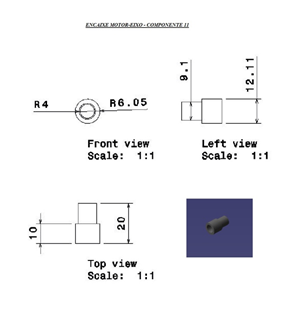
\includegraphics[scale=1.0]{figuras/tec11.png}
    \caption{Desenho Técnico componente 11}
    \label{tec11}
\end{figure}

\textbf{Componentes em y}

\begin{figure}[H]
    \centering
      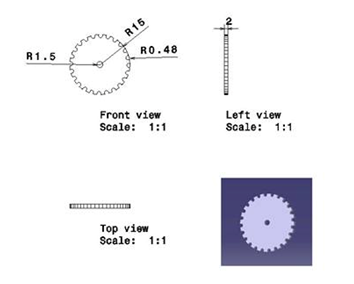
\includegraphics[scale=1.0]{figuras/tec12.png}
    \caption{Engrenagem ilustrativa para movimentação da pinça}
    \label{tec12}
\end{figure}

\begin{figure}[H]
    \centering
      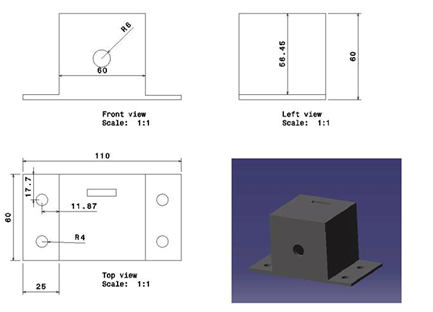
\includegraphics[scale=1.0]{figuras/tec13.png}
    \caption{Caixa para proteção de sensores}
    \label{tec13}
\end{figure}

\begin{figure}[H]
    \centering
      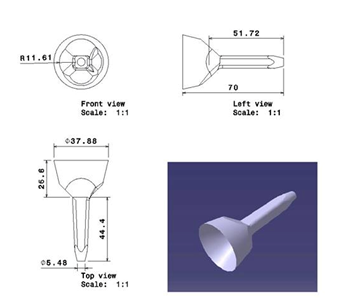
\includegraphics[scale=1.0]{figuras/tec14.png}
    \caption{Ventosa ilustrativa}
    \label{tec14}
\end{figure}

\begin{figure}[H]
    \centering
      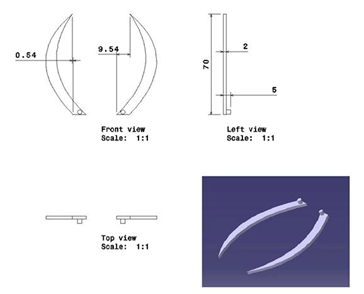
\includegraphics[scale=1.0]{figuras/tec15.png}
    \caption{Pinça da ventosa}
    \label{tec15}
\end{figure}

\chapter{Código do Processamento de Imagens - Etapa 1}

\begin{figure}[H]
    \centering
      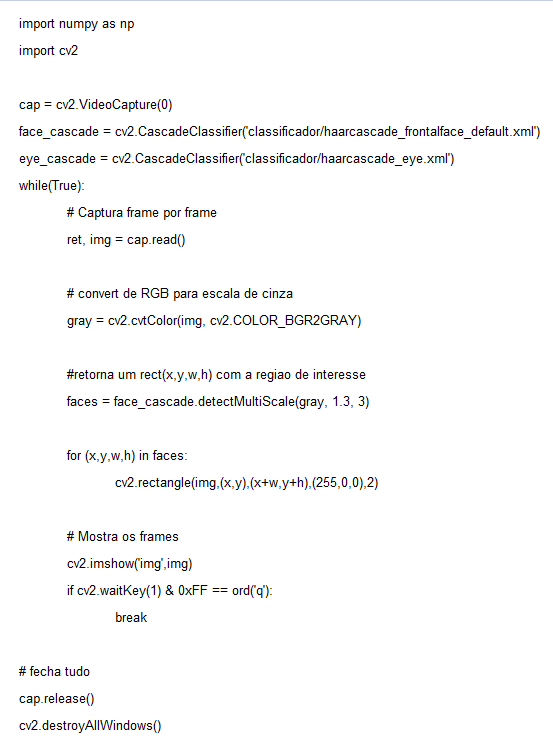
\includegraphics[scale=1.0]{figuras/img1.png}
    \label{img1}
\end{figure}

\chapter{Código do Processamento de Imagens - Etapa 2}

\begin{figure}[H]
    \centering
      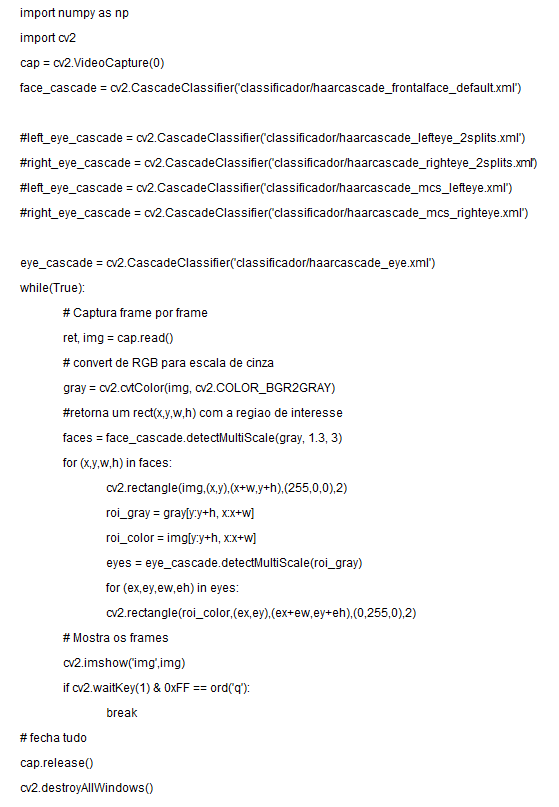
\includegraphics[scale=1.0]{figuras/img2.png}
    \label{img2}
\end{figure}

\chapter{Código do Processamento de Imagens - Etapa 3}

\begin{figure}[H]
    \centering
      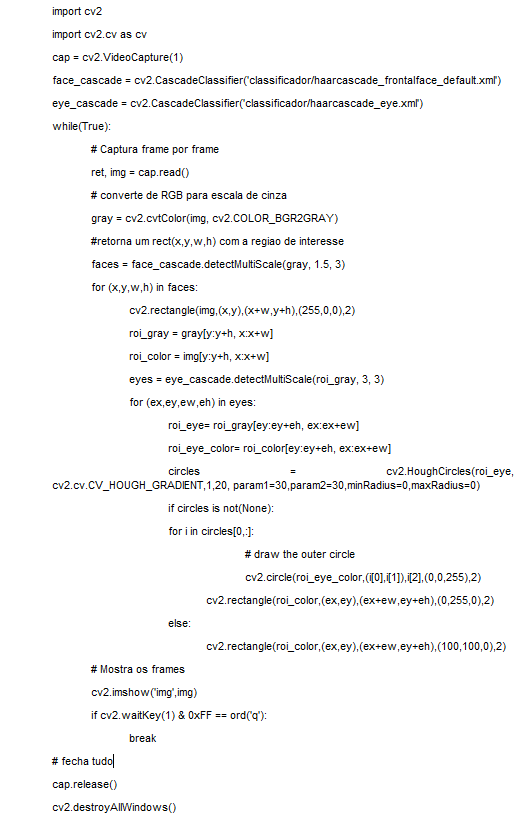
\includegraphics[scale=1.0]{figuras/img31.png}
    \label{img31}
\end{figure}




\chapter{Código da Lógica de Controle}

/*
    0: Standby -> coloca o arduino em sleepmode, interrupção tira sleepmode e diz qual comando
   
  1: Pega a lente
 
             ->função que realiza procedimento de pegar a lente retorna 1= sucesso, -1=falha

                ->move a caixinha

                ->move pra frente uma quantidade fixa de passos.

                ->move servo de pressão

                ->Testa se pegou a lente

                ->move pra trás a mesma quantidade fixa de passos

                ->Se pegou a lente retorna 1, se não pegou retorna 0.

              ->loop: enquanto função=0. 
              
    2: Move pra direta

              -> Habilita movimento do motor para direita

              -> Testa entrada do sensor óptico em um laço

              -> Para o motor
              
    3: Move pra frente

              -> abre o olho

              -> habilita interrupção de abertura de olho e toque.

              -> Move passo por passo e incrementa contador

              -> Interrupção de toque muda para o estado

              -> Interrupção de olho fechado move para o estado (PARA OU MOVE PRA TRÁS)

              -> Desabilitar a interrupção.
   
    4: Retirar/Colocar a lente a lente

              -> Testa comando.

              -> Move o servo de pressão para aplicar/desaplicar pressão

              -> Move pra trás quantidade de passos igual ao contador. 
     
    
    5: Move pra trás       

              -> recua quantidade de passos igual ao contador.

              -> incrementa contador de olhos
            
              
     
    6: Move pra esquerda

             -> Habilita movimento do motor para direita

             -> Testa entrada do sensor óptico da posição inicial em um laço

             -> Para o motor

             -> Testa contador de olhos. 
    
    7: Guarda a lente:

               ->move a caixinha

               ->move pra frente uma quantidade fixa de passos.

               ->move servo de pressão para desaplicar pressão

               ->move pra trás a mesma quantidade fixa de passos
    
   Sequência de estados para colocar a lente

         0 -> 1 -> 2 -> 3 -> 4 -> 5 -> 6 -> 1 -> 2 -> 3 -> 4 -> 5 ->6 -> 0

   Sequência para retirar lente      

         0 -> 2 -> 3 -> 4 -> 5 -> 6 -> 7 -> 2 -> 3 -> 4 -> 5 -> 6 -> 7 -> 0
     
              
*/

\#include <Servo.h>

\#include <Stepper.h>

\#include <avr/sleep.h>


//CONFIGURAÇÃO

\#define WIRES4STEPPER          //NÃO COMENTE PARA MOTOR DE PASSO DE 4 FIOS

\#define VOLTARQUANDOOLHOFECHA  //NÃO COMENTE SE MICROMOTRO DEVE VOLTAR QUANDO OLHO ABRE


//DEFINIÇÃO DE CONSTANTES

\#define PIMC 0          //Posição inicial do motor caixa

\#define PFMC 90         //Posição final do motor caixa

\#define PIMP 0          //Posição inicial do motor de pinça

\#define PFMP 90         //Posição final do motor de pinça

\#define PIMPR 0         //Posição inicial do motor de pressão

\#define PFMPR 90        //Posição final do motor de pressão

\#define SPR 200         //steps per revolution do motor de passo.

\#define SRPM 100        //RPM do stepper

\#define PASSOCAIXA      //Quantidade de passos até a caixa para pegar/guardar a lente.

\#define COMANDOTRIGGER HIGH

\#define OLHOTRIGGER HIGH

\#define TOQUETRIGGER HIGH

\#define COLOCAR  1

\#define RETIRAR  2


//PIN DEFINES

\#define PIN\_SERVO\_CAIXA 10

\#define PIN\_SERVO\_PINCA 9

\#define PIN\_SERVO\_PRESSAO 8

\#define PIN\_XR 26

\#define PIN\_XL 27

\#define PIN\_STEPPER1 22

\#define PIN\_STEPPER2 23

\#define PIN\_STEPPER3 24

\#define PIN\_STEPPER4 25

\#define PIN\_COLOCAR 2        

\#define PIN\_RETIRAR 3      

\#define PIN\_OLHO  21

\#define PIN\_TOQUE 20



Servo sservocaixa, servopinca, servopressao;

\#ifdef WIRES4STEPPER

Stepper posicionador(SPR, PIN\_STEPPER1,PIN\_STEPPER2,PIN\_STEPPER3,
PIN\_STEPPER4);

\#else

Stepper posicionador(SPR, PIN\_STEPPER1,PIN\_STEPPER2);

\#endif

int COMANDO; 

int passos=0;

int olhoaberto=1;

int contolhos=0;

void setup(){
  
    //configuração motores

    servocaixa.attach(PIN\_SERVO\_CAIXA);

    servopinca.attach(PIN\_SERVO\_PINCA);

    servopressao.attach(PIN\_SERVO\_PRESSAO);

    posicionador.setSpeed(SRPM);

    pinMode(SERVOXR,OUTPUT);

    pinMode(SERVOXL,OUTPUT);

    servocaixa.write(PIMC);

    servopinca.write(PIMP);

    servopressao.write(PIMP);

  
    //configuração dos pinos de comando

    pinMode(PIN\_COLOCAR,INPUT);

    pinMode(PIN\_RETIRAR,INPUT);

    attachInterrupt(0,,COMANDOTRIGGER);

    attachInterrupt(1,,COMANDOTRIGGER);

    
    //configuração dos pinos de sensoriamento

    pinMode(PIN\_OLHO,INPUT);

    pinMode(PIN\_TOQUE,INPUT);

  }
  
  void wakecolocar()

  {

    COMANDO=COLOCAR;

  }

  void wakeretirar()

  {

    COMANDO=RETIRAR;

  }
  
  void sleepnow(){

    set\_sleep\_mode(SLEEP\_MODE\_PWR\_DOWN);

    sleep\_enable();

    attachInterrupt(0,wakecolocar,COMANDOTRIGGER);

    attachInterrupt(1,wakeretirar,COMANDOTRIGGER);

    sleepmode();

    sleep\_disable();

    detachInterrupt(0);

    detachInterrupt(1);

  }
  
  void olhofechou(){

    olhoaberto=0;
  }
  
  void toquenoolho(){

    toque=1;

  }
  
  void loop(){ 
    
   //0 : STANDBY

   if(contolhos==0){

     passos=0;

     sleepnow(); 

   }
   
   //1 : PEGA A LENTE

   if(COMANDO==COLOCAR){

   
   }
  
   //2 : MOVE PRA DIREITA
   
   //3 : MOVE PRA FRENTE

    attachInterrupt(2,olhofechou,OLHOTRIGGER);

    attachInterrupt(3,,TOQUETRIGGER);
    
    do{

    servopinca.write(PFMP); //abre o olho - provavelmente irá mudar

    olhoaberto=1;

    toque=0;

    while((olhoaberto==1)\&\&(toque==0)){

       posicionador.step(1);

       passos++; 
    }
  

    \#ifdef VOLTARQUANDOOLHOFECHA  

      if(olhoaberto==0){

        posicionador.step(-passos);

        passos=0;

      }

    \#endif  
    

    }while(toque==0);

    detachInterrupt(2);

    detachInterrupt(3);

    
    //4 : COLOCAR/RETIRAR A LENTE

      if(COMANDO==COLOCAR){

        servopressao.write(PIMPR);

      }

      if(COMANDO==RETIRAR){

        servopressao.write(PFMPR);

      }
    

    //5 : MOVER PRA TRÁS

      posicionador.step(-passos);

      passos=0;

      contolhos++;
    

    //6 : MOVE PRA ESQUERDA

      if(contolhos>1){

        contolhos=0;
      }
   

    //7 : GUARDA A LENTE

      if(COMANDO==RETIRAR){

      }   
  
}


\chapter{Rotina para validação dos dados obtidos experimentalmente (MATLAB)}

\begin{figure}[H]
    \centering
      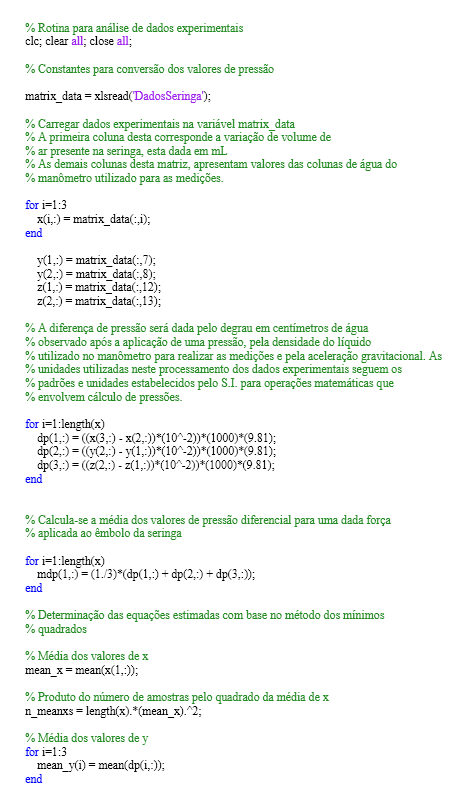
\includegraphics[scale=1.0]{figuras/rotina1.png}
    \label{rotina1}
\end{figure}

\begin{figure}[H]
    \centering
      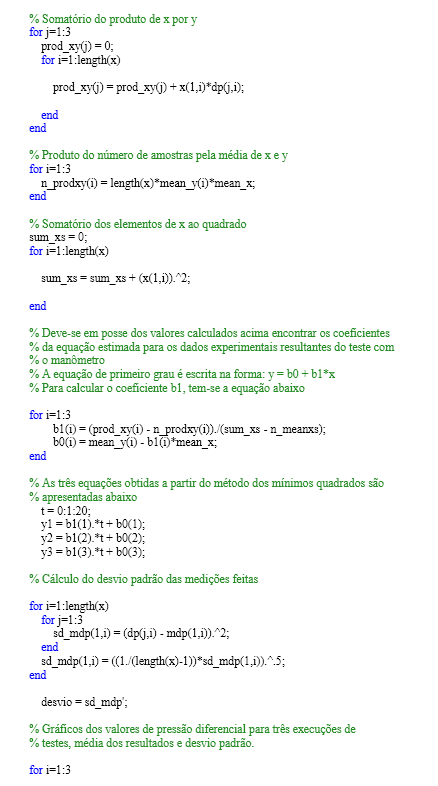
\includegraphics[scale=1.0]{figuras/rotina2.png}
    \label{rotina2}
\end{figure}

\begin{figure}[H]
    \centering
      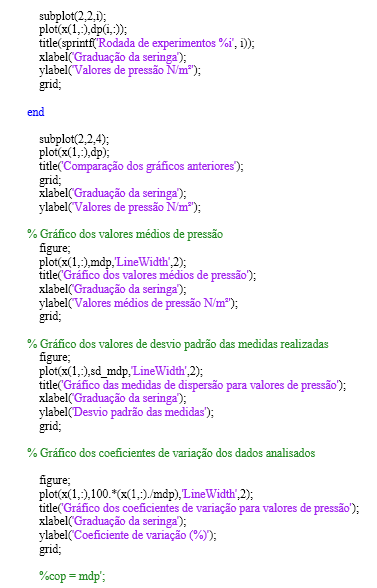
\includegraphics[scale=1.0]{figuras/rotina3.png}
    \label{rotina3}
\end{figure}




\end{apendicesenv}













